%MULTI-DIGIT MULTIPLICATION - WORKSHEET 0 (IN-CLASS INSTRUCTION)
\documentclass[12pt, letterpaper, fleqn]{article}

% ----------------------------------------------------------
% PACKAGES
% ----------------------------------------------------------
\usepackage{graphicx}
\usepackage{xcolor}
\usepackage[most]{tcolorbox}
\usepackage{amsmath, amssymb}
\usepackage{fancyhdr}
\usepackage[utf8]{inputenc}
\usepackage[T1]{fontenc}
\usepackage{enumitem}
\usepackage{geometry}
\usepackage{tikz}
\usepackage{needspace}
\usepackage{multicol}

\usetikzlibrary{arrows.meta, calc, shapes.geometric}

% ----------------------------------------------------------
% PAGE SETUP
% ----------------------------------------------------------
\usepackage{times}
\geometry{letterpaper, top=1.25in, bottom=1.25in, marginpar=0.5in}

% ----------------------------------------------------------
% HEADER / FOOTER
% ----------------------------------------------------------
\newcommand{\logowidth}{3cm}
\setlength{\headheight}{20pt}
\setlength{\footskip}{40pt}

\pagestyle{fancy}
\fancyhf{}
\fancyhead[C]{\small\bfseries Multi-Digit Multiplication}
\fancyfoot[L]{\raisebox{2pt}{
\includegraphics[width=\logowidth]{../kss.png}}}
\fancyfoot[C]{\thepage}
\fancyfoot[R]{4.9.0}

\renewcommand{\footrulewidth}{0.2pt}

% ----------------------------------------------------------
% THEME COLOR
% ----------------------------------------------------------
\definecolor{customteal}{HTML}{2fbdb9}

% ----------------------------------------------------------
% HELPER MACROS
% ----------------------------------------------------------
\newcommand{\blank}{\underline{\hspace{2.2cm}}}
\newcommand{\blanklong}{\underline{\hspace{6.5cm}}}
\newcommand{\blankshorter}{\underline{\hspace{1.5cm}}}

% ----------------------------------------------------------
% DOCUMENT
% ----------------------------------------------------------
\begin{document}

\textbf{Name:} \underline{\hspace{5cm}}
\hfill
\textbf{Date:} \underline{\hspace{3cm}}\\

\begin{tcolorbox}[colback=customteal!20]
    \large\textcolor{black}{\textbf{Multi-Digit Multiplication: Area Models}}
\end{tcolorbox}

\vspace{3mm}
\noindent
We can use an **Area Model** to break down large multiplication problems into smaller, easier pieces.
For example, to multiply $24 \times 13$:
\[
24 = 20 + 4 \qquad 13 = 10 + 3
\]

\begin{center}
\begin{tikzpicture}[scale=0.8]
\draw[thick] (0,0) rectangle (5,3);
\draw[thick] (3.5,0) -- (3.5,3);
\draw[thick] (0,1) -- (5,1);

\node[above] at (1.75,3) {20};
\node[above] at (4.25,3) {4};
\node[left] at (0,2) {10};
\node[left] at (0,0.5) {3};

\node at (1.75,2) {$20 \times 10 = 200$};
\node at (4.25,2) {$4 \times 10 = 40$};
\node at (1.75,0.5) {$20 \times 3 = 60$};
\node at (4.25,0.5) {$4 \times 3 = 12$};
\end{tikzpicture}
\end{center}
Now, add the partial products: $200 + 40 + 60 + 12 = 312$.

\newpage
\begin{tcolorbox}[colback=customteal!20]
    \large\textcolor{black}{\textbf{Guided Practice}}
\end{tcolorbox}

\vspace{5mm}
\begin{enumerate}[itemsep=4.5cm, leftmargin=0.6cm]
\item Fill in the area model to solve $35 \times 12$.
\begin{center}
\begin{tikzpicture}[scale=0.8]
\draw[thick] (0,0) rectangle (5,3);
\draw[thick] (3.5,0) -- (3.5,3);
\draw[thick] (0,1) -- (5,1);
\node[above] at (1.75,3) {30};
\node[above] at (4.25,3) {5};
\node[left] at (0,2) {10};
\node[left] at (0,0.5) {2};
\end{tikzpicture}
\end{center}
Sum of partial products: \blank $+$ \blank $+$ \blank $+$ \blank $=$ \blank

\item Solve using the standard algorithm: $143 \times 5$.
\end{enumerate}

\end{document}
